\section{Analyse bivariée}

\begin{frame}
	\begin{itemize}
	\item Même Données entrantes
	
	\begin{itemize}
		\item 814 rapport, avec les précurseurs de risque. 
		\item On a aussi obtenu les valeurs de l'evenement en pire cas, avec un deplacement spatio-temporel.
	\end{itemize}	
	
	\item On recalcule la valeur des $RR_p$ en cas des pire risque
	\item On recalcule la valeur des $R_{rapport_t}$ en cas des pire risque
	\item On fait le graphique des valeur des risque en pire cas en fonction des risques reels.

	\end{itemize}

\end{frame}

\begin{frame}
	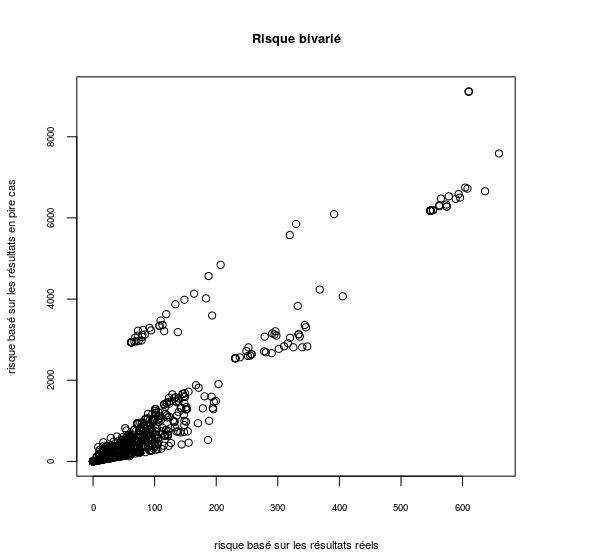
\includegraphics[width=220px, height=220px]{risque_bivarie}	
\end{frame}


\begin{frame}
	L'auteur suggère aussi une correspondance entre une valeur de risque 
	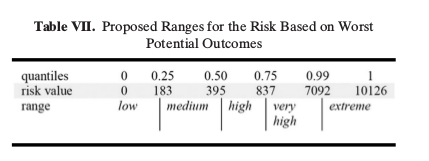
\includegraphics[width=\paperwidth]{range_propose_pire}	
\end{frame}


\begin{frame}
	Si on enleve l'effet de la fonction de répartition dans les données et qu'on ordonne chaque point selon son rang dans le jeu de donnes on obtient
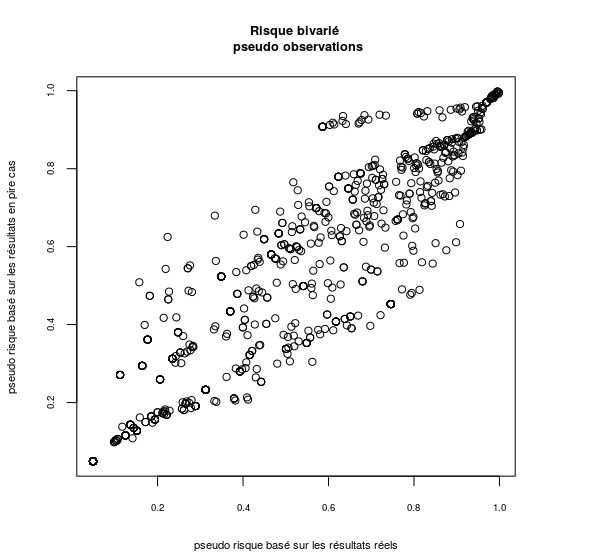
\includegraphics[width=220px, height=220px]{pseudo_risque_bivarie}	
	
\end{frame}



\item On recréer des simulations grâce à la méthode bootstrap 
\item On fait une analyse bivariée des risques
